%%
% 第四章节
\chapter{实验设计与实验分析}

\noindent
本章围绕对数梅尔频谱输入条件下的语音情绪识别实验展开，比较对象包括卷积神经网络基线模型、纯Transformer模型、窗口Transformer模型以及CNN-Conformer模型。前文已经分别介绍了语音信号处理方法、注意力机制与Transformer相关结构，因此本章不再重复相关理论，而是将重点放在实验对象、结构实现、训练设置以及结果分析之上。

\noindent
本章的实验内容可以分为两个层面。第一个层面是不同模型结构在统一输入表示与评价指标下的综合比较，第二个层面是围绕CNN-Conformer模型所开展的结构调整与过拟合缓解分析。后续各节将依次说明实验参数与模型结构、综合实验结果、噪声条件下的观察、跨语料库相关实验设想以及更细粒度的结果分析。

\section{实验参数与设置}

\subsection{数据集与任务设置}

\noindent
本章实验继续采用RAVDESS语音情绪数据集。RAVDESS语音情绪数据集包含多个情绪类别，并覆盖不同用户的语音样本，能够为用户无关条件下的语音情绪识别实验提供较为统一的测试环境。考虑到前文已经对数据集来源、类别构成以及语料特点进行了说明，本节仅保留与实验实现直接相关的设置内容。

\noindent
在任务设定方面，本文将所有模型置于相同的数据划分原则下进行比较，以尽量降低由数据切分方式带来的额外差异。实验过程中采用用户级划分思路，使训练集与验证集、测试集之间保持用户层面的分离，从而考察模型在未见用户语音上的泛化表现。上述划分设定与本文关注的实际应用情境较为一致，因为真实场景下的系统通常需要面对未参与训练的用户输入。结合实际日志可以看到，当前实验所使用的语音子集共包含1440条语音样本、24名用户，每名用户包含60条语音；8个情绪类别中，类别“01”对应96条样本，其余7个类别各包含192条样本。

% [한국어 주석] 실제 수치 확인 후 아래 표의 占位 내용을 교체하면 됨.
\begin{table}[htbp]
    \centering
    \caption{数据集构成与用户无关划分方式}
    \label{tab:chapter4_dataset_split}
    \begin{tabular}{cccc}
        \toprule
        项目 & 说明 & 数值/类别数 & 备注 \\
        \midrule
        数据集 & RAVDESS Speech & 1440条语音 & 仅使用语音部分 \\
        用户数量 & 用户01--24 & 24名用户 & 每名用户60条样本 \\
        情绪类别 & 8类 & 01--08 & 01类96条，其余各192条 \\
        划分方式 & 用户无关划分 & 5折交叉验证 & Optuna阶段通常运行1折筛选 \\
        \bottomrule
    \end{tabular}
\end{table}

\subsection{输入表示与预处理流程}

\noindent
所有比较模型均以对数梅尔频谱作为输入表示。采用对数梅尔频谱的主要原因在于，对数梅尔频谱能够在保持频谱结构信息的同时，对语音中的能量分布与频带差异提供较为稳定的刻画。与直接使用原始波形相比，对数梅尔频谱在当前数据规模下更有利于统一输入维度，也便于不同模型结构之间的对照实验。根据公开数据说明，RAVDESS原始音频为16bit、48kHz单声道语音，但本项目训练时统一重采样到16kHz，以便与当前深度学习实验配置保持一致。

\noindent
具体实现中，首先对原始语音进行重采样与幅值归一化处理，随后按照固定帧长与帧移提取时频表示，并映射到梅尔滤波器组上，最终获得对数梅尔频谱特征。对于输入长度不一致的问题，本文采用分块处理方式，将较长语音切分为多个局部片段并在推理阶段进行聚合，以减少由时长差异带来的训练不稳定现象。这一处理流程既保留了语音局部变化信息，也控制了模型训练时的显存开销。

\noindent
在数据增强方面，实验中保留了有限度的时频遮挡设置，并对增强强度进行了约束。这样处理的原因在于，前期实验表明过强的数据增强并未稳定改善验证结果，部分设置反而会削弱情绪相关细节的保留。因此，本章在综合实验中主要采用较为克制的增强策略，以避免增强幅度本身成为主要影响因素。

% [한국어 주석] waveform -> 对数梅尔频谱 -> chunk切分 -> 模型输入 흐름을 이 그림 위치에 넣으면 됨.
\begin{figure}[htbp]
    \centering
    \fbox{\parbox{0.88\textwidth}{
        \vspace{1.5cm}
        \centering
        图像占位：语音情绪识别实验的输入处理流程

        原始语音 $\rightarrow$ 重采样与归一化 $\rightarrow$ 对数梅尔频谱 $\rightarrow$ 分块处理 $\rightarrow$ 模型输入
        \vspace{1.5cm}
    }}
    \caption{语音情绪识别实验的输入处理流程}
    \label{fig:chapter4_input_pipeline}
\end{figure}

\begin{table}[htbp]
    \centering
    \caption{输入表示与预处理参数设置}
    \label{tab:chapter4_preprocess}
    \begin{tabular}{cccc}
        \toprule
        参数类别 & 参数名称 & 当前设置 & 说明 \\
        \midrule
        音频处理 & 采样率 & 16000Hz & 所有实验统一 \\
        特征提取 & n\_fft / hop\_length & 1024 / 160 & 主实验固定设置 \\
        特征维度 & Mel频带数 & 80 & CNN-Conformer与窗口Transformer主线统一 \\
        分块设置 & chunk长度/步长 & 48 / 12 & 综合实验主线常用设置 \\
        数据增强 & 时频遮挡 & 关闭或弱增强 & 最终最优方案主要依赖混合增强 \\
        \bottomrule
    \end{tabular}
\end{table}

\subsection{比较模型的结构设计}

\subsubsection{卷积神经网络基线模型}

\noindent
卷积神经网络基线模型作为本文的基础比较对象，卷积神经网络基线模型的核心思路是在二维时频平面上逐层提取局部模式，再通过池化与分类头完成情绪类别判别。卷积神经网络基线模型具有明确的局部感受野与参数共享机制，能够较为直接地学习能量突变、频带形状以及局部时频纹理等模式。在对数梅尔频谱输入条件下，这类结构通常能够形成较为稳定的训练过程，因此适合作为后续Transformer系列模型的参照对象\cite{peng2021efficient,zhang2023cnn}。

\noindent
本文采用的卷积神经网络基线模型保持了相对简洁的主干结构，不额外叠加过深的残差层或复杂注意力模块。这样处理的原因在于，本研究的目标并非追求卷积结构本身的最大化复杂度，而是以一个实现稳定、易于复现的卷积神经网络基线模型作为比较起点，从而观察Transformer系列模型在相同输入条件下是否能够取得更有意义的性能变化。需要说明的是，该模型并非单一先行研究的逐层复现，而是结合语音情绪识别中常见二维卷积结构后形成的项目内部基线实现\cite{peng2021efficient,zhang2023cnn}。

\noindent
从具体实现流程看，卷积神经网络基线模型通常由若干卷积块、非线性激活层、池化层以及分类头构成。输入的对数梅尔频谱首先进入卷积块以提取局部时频模式，再通过逐层池化压缩特征图尺寸，随后将高层特征送入全连接分类器完成情绪类别判别。卷积神经网络基线模型的结构路径相对直接，便于观察卷积局部建模在本文任务中的实际作用范围。

\noindent
本章采用的卷积神经网络基线模型代表配置来自当前最佳试验。该配置包含4个卷积块，每个卷积块均由$3 \times 3$卷积、BatchNorm、ReLU以及$2 \times 2$最大池化组成；通道数依次为$[32, 64, 256, 512]$，卷积主干之后使用AdaptiveAvgPool2d将特征图压缩为$4 \times 4$，再经Flatten、丢弃层和线性分类器输出8类情绪结果。

% [한국어 주석] CNN baseline은 다른 모델과 별도 그림으로 두는 편이 적절함.
% [한국어 주석] 내용: 4개 Conv block(각 block = 3x3 Conv + BN + ReLU + 2x2 MaxPool), AdaptiveAvgPool2d(4x4), Flatten, Dropout, Linear(8-class)
\begin{figure}[htbp]
    \centering
    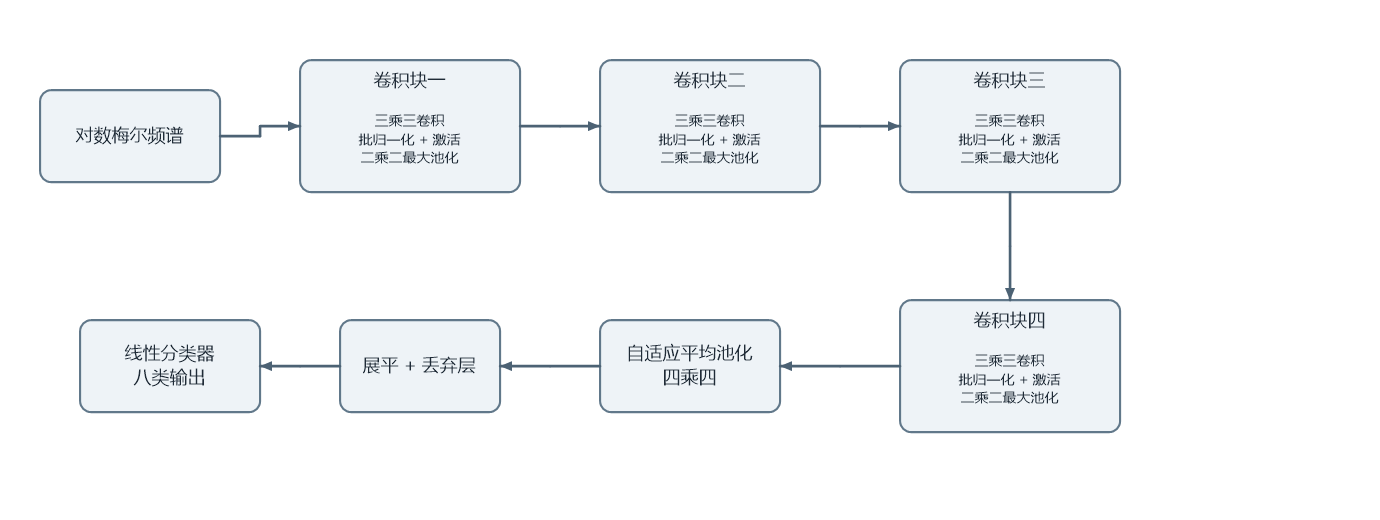
\includegraphics[width=0.97\textwidth]{images/chapter4_v1_models/cnn_baseline_architecture.png}
    \caption{卷积神经网络基线模型结构}
    \label{fig:chapter4_cnn_baseline_arch}
\end{figure}

\subsubsection{纯Transformer模型}

\noindent
纯Transformer模型不在前端引入卷积特征提取模块，而是将输入时频表示映射为一系列序列化特征后，主要依赖自注意力机制建模全局上下文关系。纯Transformer结构的优势在于能够较为直接地刻画远距离位置之间的相关性，并在统一的注意力框架下完成特征聚合。对于语音情绪识别任务而言，这种建模方式有助于观察纯全局建模策略在中小规模情绪语音数据上的表现边界\cite{vaswani2017attention}。

\noindent
与卷积神经网络基线模型相比，纯Transformer模型减少了显式局部归纳偏置，对输入表示和训练稳定性的要求相对更高。将其纳入本章比较的目的，主要在于验证当模型主要依赖全局关系建模时，是否能够充分利用语音中的情绪线索，以及这种结构在当前数据规模下是否容易受到过拟合或局部细节捕获不足的影响。这里所说的“纯Transformer模型”并不是原始机器翻译任务中的完整编码器-解码器结构，而是依据原始Transformer编码器思想改写得到的面向语音情绪分类的仅编码器结构\cite{vaswani2017attention}。

\noindent
在实现上，纯Transformer模型通常先将输入特征映射为一系列时序标记，再叠加位置编码信息，以保留不同时间位置的相对关系。随后，模型通过多头自注意力模块与前馈网络交替堆叠，对序列内部的相关性进行建模，并通过池化或分类标记完成整体判别。对于缺少卷积前端的结构而言，输入标记的组织方式、位置表示以及编码层深度都会直接影响模型对情绪细节的保持能力。

\noindent
结合当前最佳试验配置，纯Transformer模型在本项目中的代表设置为：嵌入维度256，注意力头数4，编码层数5，前馈维度1024，二维分块尺寸为$32 \times 32$，二维分块步长为$8 \times 8$，池化方式为均值池化，丢弃层比例约为0.2707。该结构直接将谱图划分为二维分块，再通过卷积形式的分块嵌入映射为标记序列。

% [한국어 주석] pure transformer는 별도 그림이 있는 편이 적절함.
% [한국어 주석] 내용: patch embedding(conv2d), positional encoding, TransformerEncoder x5, mean pooling, linear classifier
\begin{figure}[htbp]
    \centering
    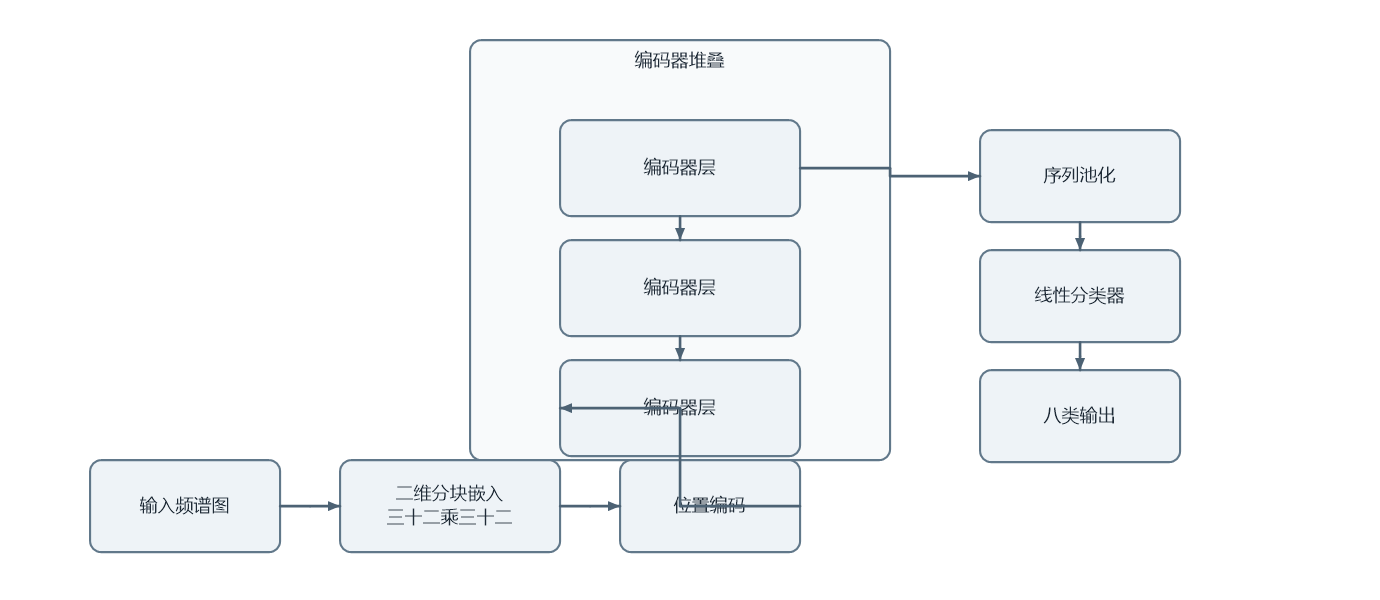
\includegraphics[width=0.97\textwidth]{images/chapter4_v1_models/pure_transformer_architecture.png}
    \caption{纯Transformer模型结构}
    \label{fig:chapter4_pure_transformer_arch}
\end{figure}

\begin{figure}[htbp]
    \centering
    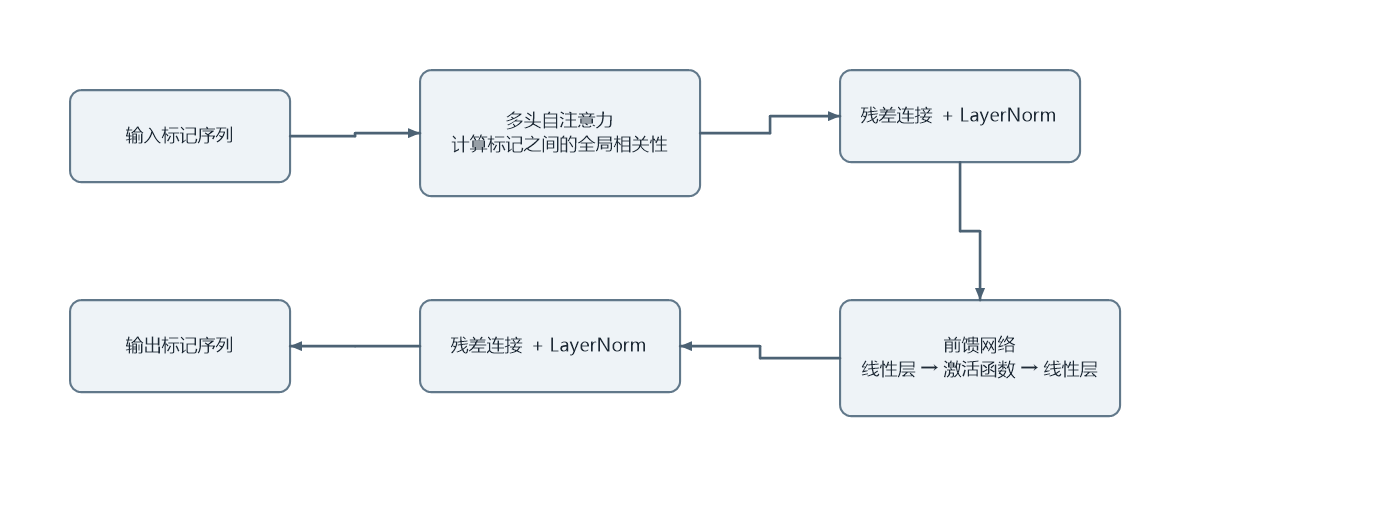
\includegraphics[width=0.97\textwidth]{images/chapter4_v1_models/transformer_encoder_block.png}
    \caption{Transformer编码器层结构}
    \label{fig:chapter4_transformer_encoder_block}
\end{figure}

\noindent
图\ref{fig:chapter4_pure_transformer_arch}与图\ref{fig:chapter4_transformer_encoder_block}对应了纯Transformer模型从谱图到句级表示的完整路径以及单层编码器的内部结构。与原始Transformer论文中的编码器-解码器框架不同，本文实现不引入解码器分支，而是保留分块嵌入、位置编码、编码器堆叠、序列池化与线性分类器五个部分，用于直接完成8类情绪判别。该处理方式使纯Transformer模型能够作为“仅依赖全局注意力建模”的代表结构，与卷积结构和卷积-注意力混合结构形成清晰对照\cite{vaswani2017attention}。

\subsubsection{窗口Transformer模型}

\noindent
窗口Transformer模型是在纯Transformer模型基础上引入局部窗口机制的代表结构。窗口Transformer模型的主要思路是将注意力计算限制在相对局部的时频区域内，以减小全局自注意力的计算负担，同时增强模型对邻近局部结构的关注。对于语音情绪识别任务而言，这类窗口化处理可以在一定程度上缓解纯Transformer模型对全局关系过度依赖的问题，并保留更清晰的局部时频模式\cite{wang2024swin,chen2023dwformer}。

\noindent
本文在综合实验中仅保留一种窗口Transformer模型作为代表比较对象，而不再同时展开多个窗口变体。这样处理的考虑在于，本研究的核心比较并不在于不同窗口家族内部的横向竞争，而是关注卷积结构、纯Transformer结构、窗口化Transformer结构与CNN-Conformer结构之间的总体差异。保留一个代表性的窗口Transformer模型，有助于控制模型种类数量，也使后续结果分析更加集中。本文所采用的桥接式窗口Transformer并不是对 Speech Swin-Transformer 或 DWFormer 的直接复现，而是在层级窗口骨干上加入桥接上下文路径后的变形实现\cite{wang2024swin,chen2023dwformer}。

\noindent
从结构流程看，窗口Transformer模型一般先将输入特征划分为若干局部窗口，再在窗口内部执行多头注意力计算，以获得局部区域内更细致的关联表示。若模型包含窗口迁移或窗口间信息交换模块，则不同局部区域之间的关系会在后续层中逐步建立。窗口Transformer结构与纯Transformer模型相比，更强调相邻时频区域的局部组织方式，因此适合用于观察局部窗口约束是否能够缓解纯全局建模带来的训练不稳定问题。

\noindent
考虑到窗口模型家族内部已经进行过多次变体探索，本章综合实验只保留桥接式窗口Transformer作为窗口Transformer模型的代表。当前最佳窗口Transformer配置为：前端卷积通道$[48, 64]$，两个阶段的隐藏维度分别为96与160，阶段深度分别为3与2，对应注意力头数分别为4与8，窗口大小分别为$[4,8]$与$[5,8]$，前馈扩展比为3.0，桥接标记数量为2，池化方式为均值池化，丢弃层比例约为0.1008。该模型同时包含相对位置偏置、移位窗口以及桥接上下文注入路径。

% [한국어 주석] window transformer는 별도 그림이 권장됨.
% [한국어 주석] 내용: ConvStemBlock x2 -> SpatialProjector -> Stage1(3 blocks, shifted window) -> BridgeContext -> PatchMerging -> Stage2(2 blocks) -> Bridge fusion -> mean pooling -> classifier
\begin{figure}[htbp]
    \centering
    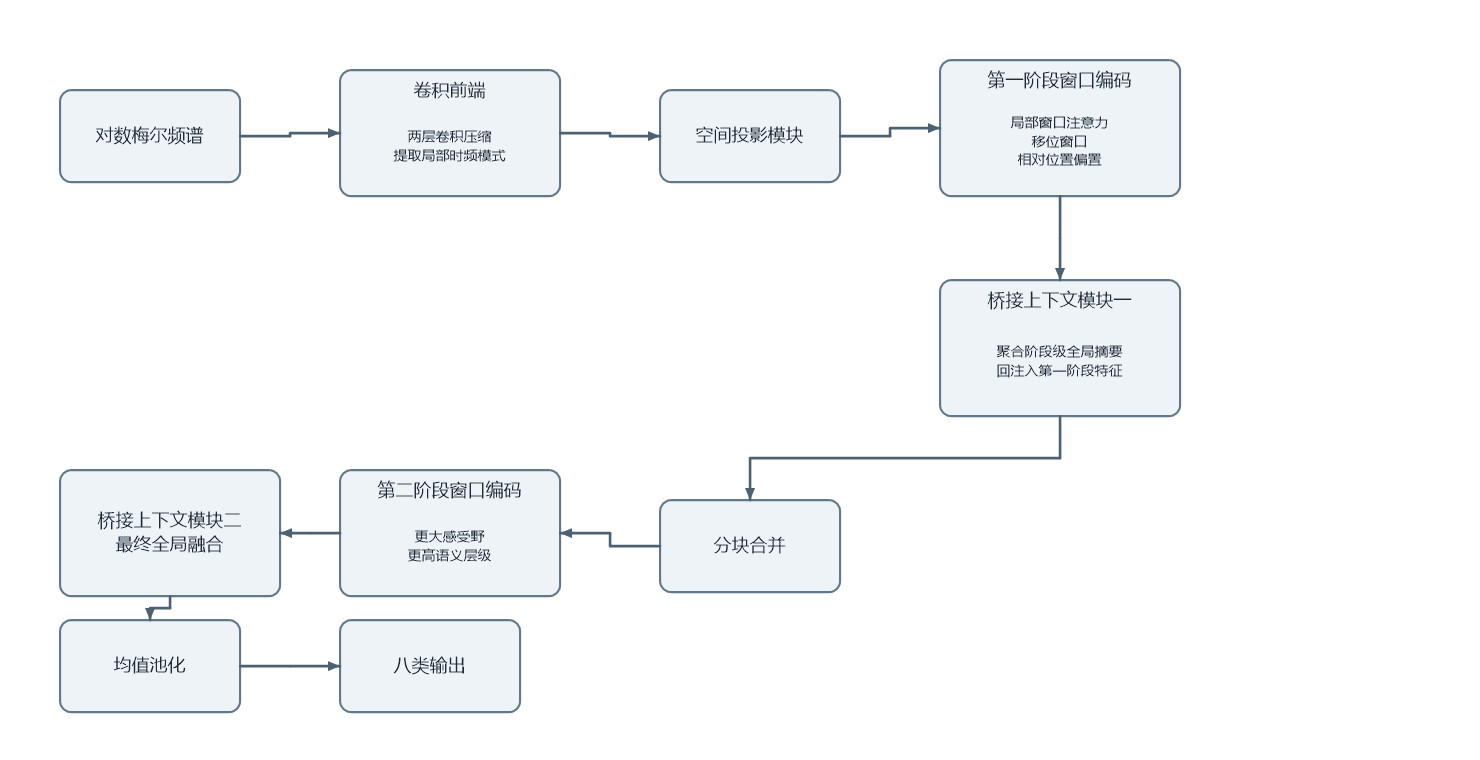
\includegraphics[width=0.99\textwidth]{images/chapter4_v1_models/bridged_window_transformer_architecture.png}
    \caption{窗口Transformer模型结构}
    \label{fig:chapter4_window_transformer_arch}
\end{figure}

\noindent
图\ref{fig:chapter4_window_transformer_arch}给出了本文窗口Transformer模型的主干流程。该结构在Speech Swin-Transformer的层级窗口注意力基础上，进一步加入桥接上下文路径，用于在不同阶段之间回注入全局情绪摘要。就具体实现而言，前端卷积模块负责局部时频压缩，第一阶段与第二阶段分别执行窗口注意力与移位窗口建模，桥接上下文模块负责跨窗口的摘要提取与重加权，末端通过均值池化与线性分类器完成8类情绪输出。与纯Transformer模型相比，这一路径显式保留了局部窗口归纳偏置；与标准Swin式骨干相比，又额外加入了面向语音情绪任务的全局上下文补偿支路\cite{wang2024swin,chen2023dwformer}。

\noindent
图\ref{fig:chapter4_window_transformer_arch}中的“空间投影模块”对应窗口主干进入层级编码之前的维度整理步骤，其作用是将前端卷积输出变换到窗口注意力所需的统一通道空间，以便后续第一阶段与第二阶段使用一致的二维特征组织方式。“桥接上下文模块”则不是简单的命名替换，而是本文窗口模型相对标准窗口骨干的实际改写部分。该模块先将阶段特征图展平为空间标记，再引入少量可学习桥接标记作为全局查询，通过交叉注意力从全部局部标记中提取阶段级情绪摘要，随后将该摘要回注入当前阶段或下一阶段特征，从而缓解局部窗口注意力难以充分表达全局情绪上下文的问题。

\begin{figure}[htbp]
    \centering
    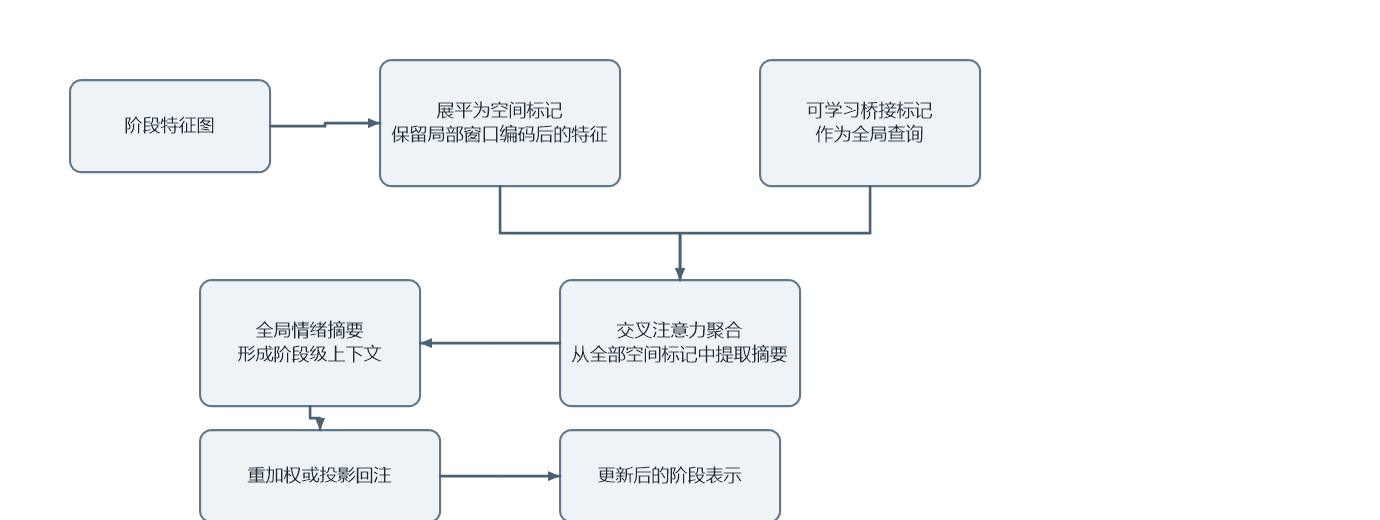
\includegraphics[width=0.99\textwidth]{images/chapter4_v1_models/bridge_context_detail.png}
    \caption{桥接上下文模块的内部逻辑}
    \label{fig:chapter4_bridge_context_detail}
\end{figure}

\subsubsection{CNN-Conformer模型}

\noindent
CNN-Conformer模型来源于卷积模块与Conformer编码器相结合的设计思路。在原始Conformer及其后续语音任务变体中，常见做法是先通过前端卷积模块完成局部变换或下采样，再将中间表示映射到统一嵌入空间，随后利用Conformer编码器联合建模局部卷积信息与全局上下文信息，最后通过池化与分类头输出类别结果\cite{gulati2020conformer,zou2022speech,peng2021efficient}。本文将这一结构家族作为重点比较对象，目的在于检验卷积归纳偏置与注意力上下文建模在语音情绪识别任务中能否形成更有效的互补关系。

\noindent
将CNN-Conformer模型作为本章重点分析对象，主要有两个原因。第一，CNN-Conformer模型在理论上兼顾了卷积结构对局部时频细节的建模能力以及注意力结构对较长上下文关系的表达能力，与本文的模型比较主线具有较强关联。第二，已有实验记录显示，CNN-Conformer模型虽然在部分设置下能够达到较高的验证准确率，但也持续暴露出过拟合倾向。因此，围绕CNN-Conformer模型开展更细致的结构调整与训练策略分析，能够更直接回应本文关于“卷积结构与Transformer结构如何在语音情绪识别中组合”的研究问题。需要说明的是，本文综合实验所采用的最优配置已不再保留原始自动语音识别场景中常见的两级卷积压缩前端，而是改为更偏向语音情绪识别场景的无卷积前端时间分块输入组织方式，这一点与原始Conformer有明确差异\cite{gulati2020conformer,zou2022speech,peng2021efficient}。

\noindent
在本文最终采用的实现中，CNN-Conformer模型的前端不再承担强压缩作用，而是先利用无卷积前端时间分块方式直接构造序列标记；中间部分由若干Conformer编码块构成，每个编码块内部包含前馈网络、多头自注意力模块、卷积模块以及残差连接；末端部分通过注意力池化形成句级表示，并交由分类头输出情绪类别。由此可以看出，当前最优实现真正承担主要建模任务的是“时间分块标记构造、Conformer序列编码、句级聚合”三个部分，而不是传统ASR式卷积下采样前端。

\noindent
当前章节在综合实验中采用的CNN-Conformer代表配置，采用后续实验中表现最强的无卷积前端时间分块输入变体。该配置中，时间块长度为4，归一化方式为LayerNorm，嵌入维度为192，编码层数为4，注意力头数为8，前馈维度为768，卷积模块卷积核大小为31，层间融合方式为末层输出，池化方式为注意力池化；训练阶段同时结合频谱级混合增强，$\alpha=0.4$。在代码实现上，Conformer块内部的执行顺序为“前馈网络$\rightarrow$相对位置多头自注意力$\rightarrow$卷积模块$\rightarrow$前馈网络$\rightarrow$LayerNorm”，并在两个前馈分支处使用0.5倍率的macaron残差结构。

\noindent
分类器设计方面，CNN-Conformer模型首先通过注意力池化获得句级嵌入，再经过丢弃层与线性层完成8类情绪分类。对于本章所采用的最优配置而言，分类器之前的句级表示维度为192，分类头结构相对简洁，目的是将性能差异更多地保留在前端标记构造方式与Conformer编码路径本身，而不是来自额外复杂的后端分类器。

\noindent
这里所说的“无卷积前端时间分块输入”并不是孤立的实验代号，而是一种专门面向情绪细粒度时间线索保留而设计的输入组织方式。该做法不再使用标准两级卷积前端先压缩时频图，而是直接使用一个覆盖全部频带、高度等于全部Mel频带数、宽度等于固定时间帧数的卷积核，将整幅谱图沿时间轴切分为若干连续时间块。每个时间块在进入序列编码之前已经包含全部频带信息，再经过层归一化和线性投影得到统一维度的序列标记。图\ref{fig:chapter4_nostem_patch_tokenization}进一步给出了这一输入组织方式的形成过程。与强时间下采样的卷积前端相比，这一路径更强调保留短时情绪变化的细粒度时间线索，适合用于检验Conformer在较弱前端压缩条件下的实际收益。

% [한국어 주석] CNN-Conformer는 반드시 단독 상세 그림을 두는 편이 좋음.
% [한국어 주석] 내용: nostem_patch(time_patch=4) -> input projection -> CNNConformerBlock x4 -> attention pooling -> dropout -> classifier
% [한국어 주석] 추가로 Conformer block 내부 세부도(FFN, relative MHSA, ConvModule, FFN, residual, norm)를 하위 그림으로 두는 것이 좋음.
\begin{figure}[htbp]
    \centering
    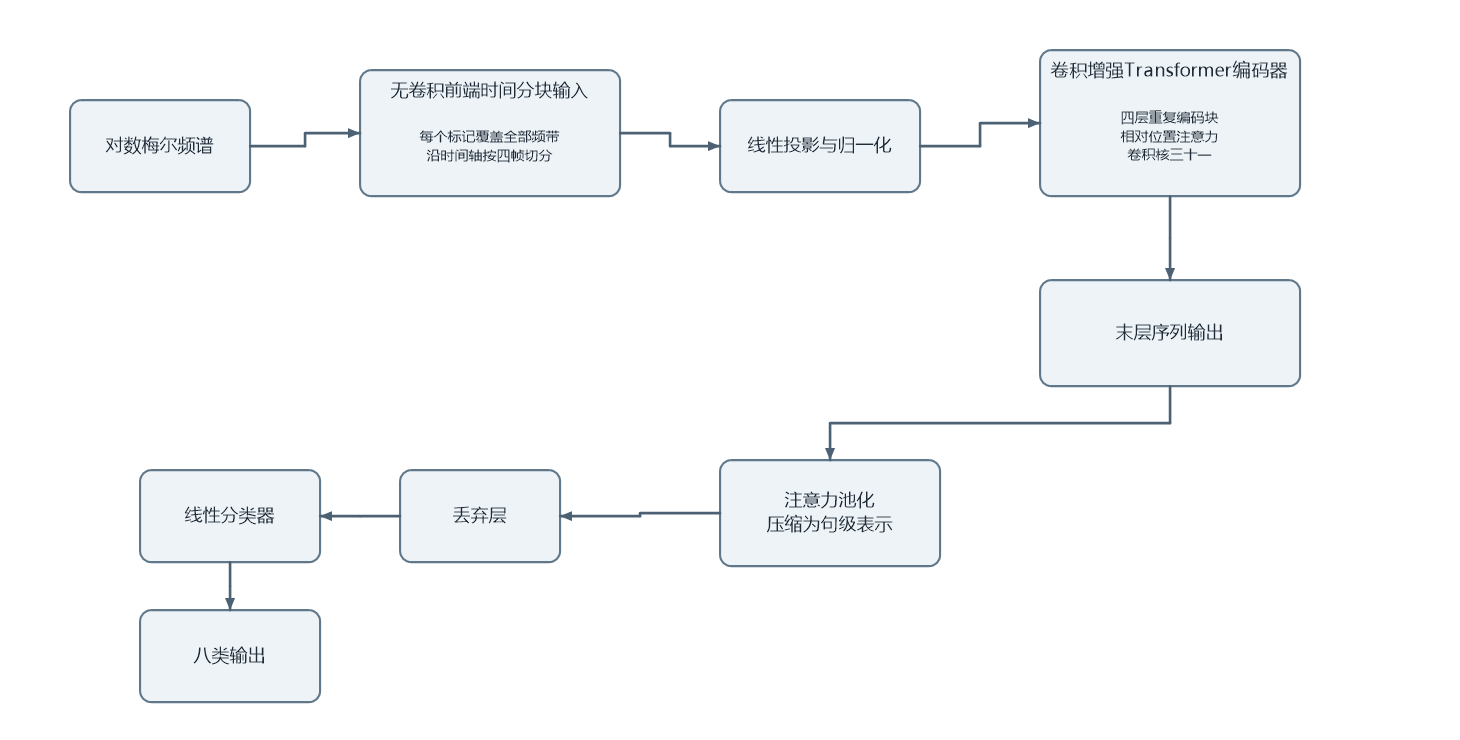
\includegraphics[width=0.97\textwidth]{images/chapter4_v1_models/cnn_conformer_architecture.png}
    \caption{CNN-Conformer模型结构}
    \label{fig:chapter4_cnn_conformer_arch}
\end{figure}

\begin{figure}[htbp]
    \centering
    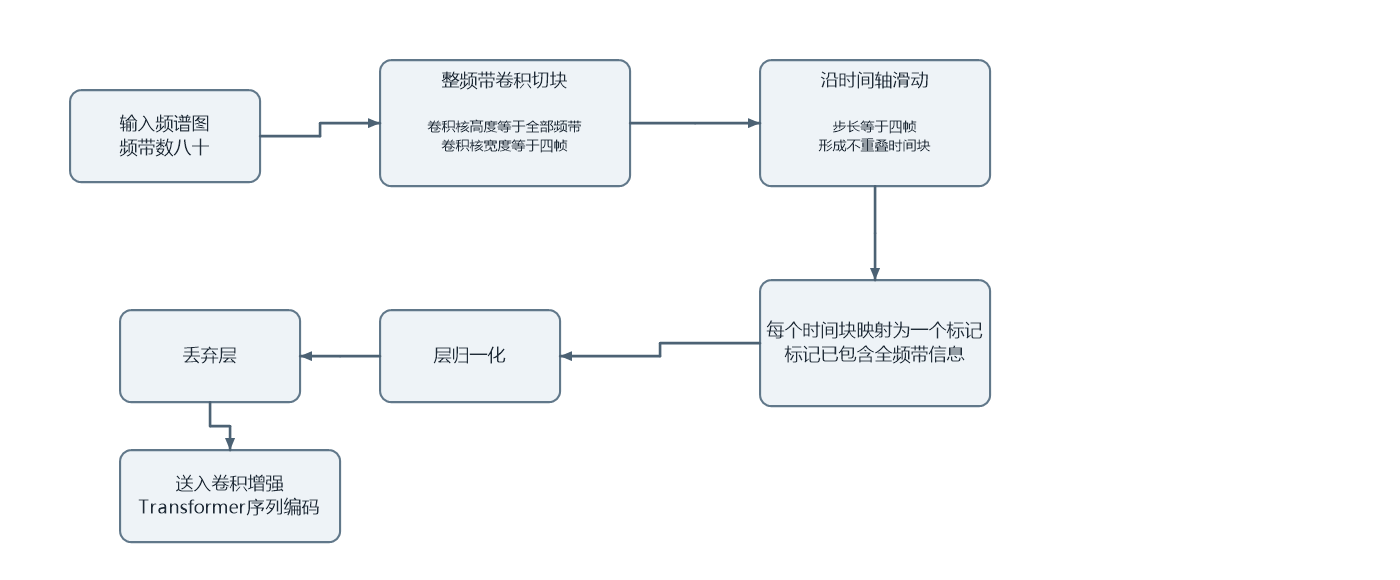
\includegraphics[width=0.97\textwidth]{images/chapter4_v1_models/nostem_patch_tokenization.png}
    \caption{无卷积前端时间分块输入的形成过程}
    \label{fig:chapter4_nostem_patch_tokenization}
\end{figure}

\begin{figure}[htbp]
    \centering
    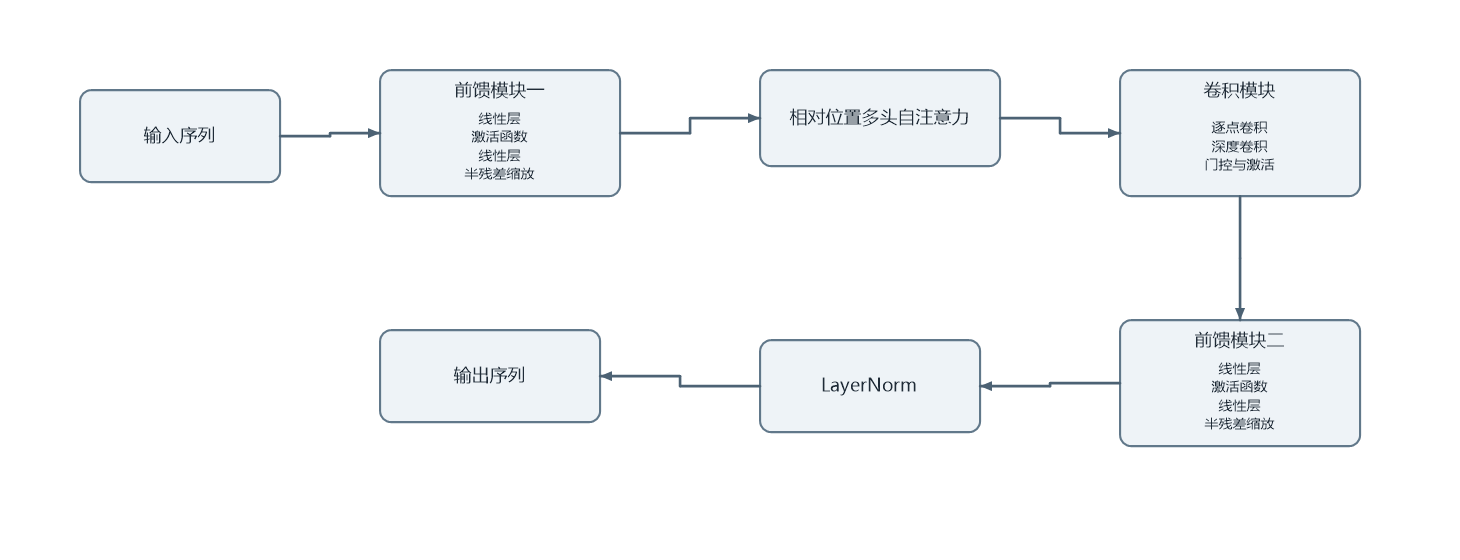
\includegraphics[width=0.97\textwidth]{images/chapter4_v1_models/conformer_block.png}
    \caption{Conformer编码块结构}
    \label{fig:chapter4_conformer_block}
\end{figure}

\noindent
图\ref{fig:chapter4_cnn_conformer_arch}、图\ref{fig:chapter4_nostem_patch_tokenization}与图\ref{fig:chapter4_conformer_block}分别对应CNN-Conformer模型的整体实现路径、无卷积前端时间分块输入的形成方式以及单个Conformer编码块的内部结构。需要说明的是，本文所采用的最佳配置并未完全照搬原始Conformer在自动语音识别任务中的前端设计，而是改为更适合语音情绪识别的无卷积前端时间分块输入组织方式，以减轻强时间压缩带来的细粒度情绪线索损失。编码阶段仍保留Conformer块中“前馈网络、相对位置多头自注意力、卷积模块、前馈网络、LayerNorm”的主干顺序，后端则使用注意力池化、丢弃层与线性分类器完成8类情绪判别，从而将结构差异集中在前端标记构造与序列编码部分\cite{gulati2020conformer,zou2022speech,peng2021efficient}。

% [한국어 주석] 네 모델의 입력-주요 모듈-출력 흐름을 한 그림에 배치하면 됨.
\begin{figure}[htbp]
    \centering
    \fbox{\parbox{0.9\textwidth}{
        \vspace{1.8cm}
        \centering
        图像占位：各比较模型的结构示意图

        卷积神经网络基线模型 / 纯Transformer模型 / 窗口Transformer模型 / CNN-Conformer模型

        建议内容：输入形式、主干结构、聚合方式、分类输出
        \vspace{1.8cm}
    }}
    \caption{各比较模型的结构示意图}
    \label{fig:chapter4_model_overview}
\end{figure}

\begin{table}[htbp]
    \centering
    \caption{各比较模型的结构差异与设计特点}
    \label{tab:chapter4_model_compare}
    \begin{tabular}{ccccc}
        \toprule
        模型 & 前端卷积 & 全局注意力 & 局部窗口机制 & 结构特点 \\
        \midrule
        卷积神经网络基线模型 & 有 & 无 & 无 & 4层卷积块后直接分类 \\
        纯Transformer模型 & 无 & 有 & 无 & 二维分块标记与编码器堆叠 \\
        窗口Transformer模型 & 有 & 有 & 有 & 两阶段移位窗口与桥接上下文 \\
        CNN-Conformer模型 & 可选 & 有 & 无 & Conformer序列编码与注意力池化 \\
        \bottomrule
    \end{tabular}
\end{table}

\subsection{训练参数与评价指标}

\noindent
为保证不同模型之间的可比性，本文尽量在统一训练框架下完成各类实验。训练过程中采用相同的数据读取流程、相近的优化策略以及一致的早停规则，并以验证集结果作为模型选择的重要依据。在参数优化方面，部分实验通过Optuna搜索学习率、批大小、分块长度以及模型内部关键参数，但本节不展开搜索日志本身，仅保留与最终对比结果直接相关的设置内容。

\noindent
评价指标主要采用准确率与宏平均F1值，同时结合UAR进行补充观察。准确率可以直接反映整体分类正确比例，宏平均F1值更适合在类别分布不完全均衡时观察模型在各类别上的平均表现，UAR则用于观察不同类别召回率的整体平衡情况。考虑到语音情绪识别任务中不同情绪类别的可分性存在差异，仅使用准确率往往不足以完整反映模型质量，因此本章在结果讨论中将同时参考上述三个指标。

\noindent
在CNN-Conformer模型的后续实验中，还引入了损失函数、采样策略、层间特征融合方式以及前端压缩方式等设置变化。保留这些变量的原因并不在于扩大搜索规模，而在于观察模型是否可以通过更贴近任务特性的结构调整缓解验证集性能波动。相关实验结果将在综合实验部分结合代表性配置进行分析。

\begin{table}[htbp]
    \centering
    \caption{训练参数与评价指标设置}
    \label{tab:chapter4_train_eval}
    \begin{tabular}{cccc}
        \toprule
        类别 & 项目 & 当前设置 & 说明 \\
        \midrule
        优化设置 & 优化器 & AdamW系配置 & 各模型统一搜索主框架 \\
        优化设置 & 学习率 & $10^{-4}$量级为主 & Optuna搜索后择优 \\
        训练设置 & 批大小 & 12或16 & 由显存与模型规模决定 \\
        训练设置 & 训练轮数 & 30轮，早停10轮 & 以验证集最优点截断 \\
        评价设置 & 指标 & Accuracy / Macro-F1 / UAR & 与结果表一致 \\
        评价设置 & 模型选择依据 & 验证集Macro-F1 & 以宏平均F1作为固定优化目标 \\
        \bottomrule
    \end{tabular}
\end{table}

\begin{table}[htbp]
    \centering
    \caption{CNN-Conformer关键搜索维度与候选设置}
    \label{tab:chapter4_conformer_search_space}
    \begin{tabular}{ccc}
        \toprule
        搜索维度 & 候选设置 & 设计目的 \\
        \midrule
        时间下采样 & 标准压缩 / 优先保留时间分辨率等 & 调整时间分辨率保留程度 \\
        层间特征融合 & 末层输出 / 可学习加权融合 & 结合浅层与深层表示 \\
        损失函数 & 交叉熵 / 焦点损失等 & 观察类别学习稳定性 \\
        采样策略 & 随机采样 / 加权采样 & 缓解类别分布差异影响 \\
        正则化设置 & 混合增强 / 丢弃层 / 归一化变体 & 控制过拟合风险 \\
        \bottomrule
    \end{tabular}
\end{table}

\section{综合实验}

\subsection{各比较模型的综合实验结果}

\noindent
在统一的输入表示、训练流程与评价指标下，四类模型的综合实验结果构成了本章分析的基础。卷积神经网络基线模型提供了较为稳定的参照性能，纯Transformer模型用于观察全局注意力建模在当前数据规模下的实际表现，窗口Transformer模型用于考察局部窗口机制是否能够在一定程度上改善纯Transformer结构的局部特征提取能力，而CNN-Conformer模型则用于验证卷积结构与注意力结构结合后是否能够形成更有效的特征表达。为保证比较具有可读性，本节使用各模型在现有实验记录中的代表性最优结果作为综合对比对象。

\noindent
从已有实验结果看，卷积神经网络基线模型在当前任务设定下仍然表现出较强的稳定性，代表结果达到Accuracy 0.61667、Macro-F1 0.62196。纯Transformer模型能够学习跨时间位置的关系，但在验证集上并未持续展现出优于卷积神经网络基线模型的优势，当前代表结果为Accuracy 0.52000、Macro-F1 0.51163。窗口Transformer模型在局部上下文建模方面表现出一定合理性，窗口Transformer模型的结果通常较纯Transformer模型更具针对性，代表结果为Accuracy 0.56333、Macro-F1 0.55338，但这种改进仍未达到卷积神经网络基线模型的水平。CNN-Conformer模型的表现介于卷积神经网络基线模型与其他Transformer系列模型之间，在部分配置下能够达到当前Transformer系列中的最高水平，当前最佳结果达到Accuracy 0.70000、Macro-F1 0.70563。

\noindent
这一现象说明，在当前数据规模与输入表示条件下，模型结构的复杂化并不会自然带来性能提升。卷积结构在局部时频模式提取方面仍然具有较强适配性，而纯Transformer结构若缺少足够明确的局部归纳偏置，则可能难以稳定捕捉情绪相关细节。窗口Transformer模型与CNN-Conformer模型虽然试图在局部建模与全局建模之间寻找平衡，但窗口Transformer模型与CNN-Conformer模型的收益仍然受到训练稳定性、参数规模以及特征压缩方式等因素的共同影响。

\begin{table}[htbp]
    \centering
    \caption{各比较模型的综合实验结果}
    \label{tab:chapter4_overall_results}
    \begin{tabular}{ccccc}
        \toprule
        模型 & Accuracy & Macro-F1 & 参数量 & 说明 \\
        \midrule
        卷积神经网络基线模型 & 0.61667 & 0.62196 & 1.41M & 4层卷积基线 \\
        纯Transformer模型 & 0.52000 & 0.51163 & 4.21M & 全局注意力建模 \\
        窗口Transformer模型 & 0.56333 & 0.55338 & 1.17M & 桥接式窗口Transformer代表结果 \\
        CNN-Conformer模型 & 0.70000 & 0.70563 & 3.55M & 当前Transformer主线最佳 \\
        \bottomrule
    \end{tabular}
\end{table}

% [한국어 주석] 종합실험 표 바로 뒤에는 필요 시 대표 artifact 1개를 넣을 수 있음.
% [한국어 주석] 후보 1: bridged window confusion matrix
% [한국어 주석] 상대경로: ../../outputs/2026-04-17/15-23-22_bridged_window_stage1_try/optuna_trials/trial_0082/artifacts/global_confusion_matrix.png
% [한국어 주석] 후보 2: CNN-Conformer winner learning curve
% [한국어 주석] 상대경로: ../../outputs/2026-04-21/18-47-36_cnn_conformer/optuna_trials/trial_0003/artifacts/fold_1_learning_curve.png

\subsection{CNN-Conformer模型的结构优化路径}

\noindent
由于CNN-Conformer模型同时包含前端卷积变换、序列编码与分类模块，CNN-Conformer模型的性能受多个结构因素共同影响。结合前期实验记录，本文围绕CNN-Conformer模型主要考察了以下几个方向：时间下采样方式、层间特征融合方式、损失函数与采样策略、前端主干结构重设计以及过拟合缓解策略。这些调整并非彼此孤立，而是围绕同一个问题展开，即如何在保持局部情绪线索的同时降低训练后期的验证性能劣化。

\noindent
在时间下采样方面，实验关注的是前端压缩对局部时间分辨率的影响。较强的时间压缩有助于降低序列长度与计算成本，但也可能压缩情绪识别所依赖的短时动态变化。基于这一考虑，后续实验逐步引入了较为温和的压缩方式，用以观察保留更多时间分辨率后模型是否能够获得更稳定的验证结果。

\noindent
在层间特征融合方面，实验尝试利用不同编码层的输出构造更丰富的表示。层间特征融合的基本思路是，将浅层较偏局部的表征与深层较偏上下文的表征进行组合，从而减轻仅使用末层输出所带来的信息单一问题。层间特征融合的有效性并不完全取决于融合是否存在，还受到编码层数、池化方式以及参数规模的影响，因此需要与其他设置一并考察。

\noindent
在训练策略方面，本文进一步考察了损失函数与采样策略的组合方式。相关调整主要服务于两个目标。第一个目标是减轻类别分布差异对训练过程的影响，第二个目标是在验证集波动较大的情况下提高模型训练的稳定性。除此之外，针对CNN-Conformer模型在后期训练中容易出现训练准确率持续上升而验证结果停滞甚至回落的现象，实验还引入了主干结构重设计以及更克制的正则化调节，以观察模型容量与过拟合风险之间的关系。

\begin{figure}[htbp]
    \centering
    \fbox{\parbox{0.9\textwidth}{
        \vspace{1.8cm}
        \centering
        图像占位：CNN-Conformer模型的结构优化路径

        初始结构设定 $\rightarrow$ 时间下采样调整 $\rightarrow$ 层间特征融合

        $\rightarrow$ 损失函数与采样策略 $\rightarrow$ 主干重设计 $\rightarrow$ 过拟合缓解
        \vspace{1.8cm}
    }}
    \caption{CNN-Conformer模型的结构优化路径}
    \label{fig:chapter4_conformer_path}
\end{figure}

\subsection{CNN-Conformer模型的最终配置与结果观察}

\noindent
在综合比较层面，CNN-Conformer模型的最终配置并不是由单一参数直接决定，而是在多个候选方向之间逐步筛选形成的。现有实验结果表明，较温和的时间下采样方式、有限度的层间特征融合、适度的损失函数调整以及较为克制的正则化设置，通常更有助于得到相对稳定的验证结果。相较于一味增加模型容量，这类以保留信息和控制过拟合为目标的调整，更符合当前数据规模下的训练需求。当前最佳结果对应的代表配置采用无卷积前端时间分块输入、时间块长度为4、LayerNorm归一化、4层Conformer编码器、8头注意力、卷积核大小31以及注意力池化，并在训练时加入$\alpha=0.4$的混合增强。

\noindent
与此同时，需要注意的是，CNN-Conformer模型虽然在部分配置上能够达到约0.7左右的准确率水平，但其训练曲线仍然多次呈现出训练集指标持续提升而验证集指标提前停止改善的情况。这一现象说明，模型已经具备较强的训练集拟合能力，但对未见用户语音的泛化能力仍然有限。由此可以看出，CNN-Conformer模型的后续优化重点不应仅停留在扩大结构复杂度上，而更需要关注特征压缩方式、模型容量控制以及训练策略之间的平衡。

\noindent
从比较结果来看，CNN-Conformer模型的价值主要体现在两个方面。一方面，卷积结构与注意力结构的结合并非没有意义，在适当设置下确实能够获得比纯Transformer模型更具竞争力的结果；另一方面，卷积与注意力结合结构在中小规模语音情绪数据上面临的共同问题也较为明显，即更强的表达能力往往伴随着更高的过拟合风险。因此，后续分析不宜仅以“更复杂”作为优化方向，而应进一步检视模型中哪些部分真正对泛化能力产生了稳定贡献。

\begin{table}[htbp]
    \centering
    \caption{CNN-Conformer模型的最终配置}
    \label{tab:chapter4_conformer_final}
    \begin{tabular}{ccc}
        \toprule
        配置维度 & 最终设置 & 备注 \\
        \midrule
        前端形式 & 无卷积前端时间分块输入，时间块长度为4 & 不使用标准两级卷积前端 \\
        层间特征融合 & last & 采用末层输出 \\
        损失函数 & 交叉熵 & 标签平滑设为0 \\
        采样策略 & random & 不额外使用加权采样 \\
        池化方式 & attention & 句级表示由注意力池化获得 \\
        正则化设置 & 混合增强 $\alpha=0.4$ + 丢弃层 & LayerNorm，未采用缩窄策略 \\
        \bottomrule
    \end{tabular}
\end{table}

\begin{table}[htbp]
    \centering
    \caption{CNN-Conformer模型阶段性结果汇总}
    \label{tab:chapter4_conformer_stage_results}
    \begin{tabular}{ccccc}
        \toprule
        优化阶段 & 主要改动 & 最佳Accuracy & 最佳Macro-F1 & 现象 \\
        \midrule
        初始结构设定 & 标准两级卷积前端 + 相对位置Conformer & 0.63000 & 0.63168 & 形成早期最优基线 \\
        时间下采样调整 & 保留更多时间分辨率 & 0.62017 & 0.62017 & 有一定价值但未超越早期最优基线 \\
        层间特征融合 & 末层输出与加权融合比较 & 0.55348 & 0.55348 & 第二轮探索未形成突破 \\
        训练策略调整 & 损失函数 / 采样策略 / 混合增强 & 0.70000 & 0.70563 & 混合增强路线达到全局最佳 \\
        主干与正则化调整 & 无卷积前端时间分块输入 + 归一化筛选 & 0.70333 & 0.70042 & 最后一轮结果接近最佳但未超越 \\
        \bottomrule
    \end{tabular}
\end{table}

% [한국어 주석] 필요하다면 train/val curve 대표 artifact를 이 위치 뒤에 넣으면 됨. 과적합을 보여주는 대표 사례 1개 정도가 적절함.
% [한국어 주석] 추천 상대경로:
% [한국어 주석] 1) 최고 CNN-Conformer learning curve
% [한국어 주석] ../../outputs/2026-04-21/18-47-36_cnn_conformer/optuna_trials/trial_0003/artifacts/fold_1_learning_curve.png
% [한국어 주석] 2) 최고 CNN-Conformer attention map
% [한국어 주석] ../../outputs/2026-04-21/18-47-36_cnn_conformer/optuna_trials/trial_0003/artifacts/fold_1_attention_map.png
% [한국어 주석] 3) 최고 CNN-Conformer cnn feature map
% [한국어 주석] ../../outputs/2026-04-21/18-47-36_cnn_conformer/optuna_trials/trial_0003/artifacts/fold_1_cnn_feature_map.png

\subsection{综合讨论}

\noindent
从整体比较结果可以看到，在当前实验条件下，卷积神经网络基线模型仍然构成一个难以忽略的参照基线。出现这一结果并不一定意味着卷积结构在所有条件下都优于Transformer结构，而更可能说明在数据规模有限、输入表示相对固定的语音情绪识别任务中，明确的局部归纳偏置仍然具有较高实用价值。纯Transformer模型虽然具备较强的全局关系建模能力，但若缺少与任务相匹配的局部约束，纯Transformer模型的优势未必能够充分转化为验证集上的稳定收益。

\noindent
窗口Transformer模型与CNN-Conformer模型分别从两种不同方向尝试弥补这一不足。窗口Transformer模型通过限制注意力范围增强局部区域建模，CNN-Conformer模型则直接在卷积特征提取与注意力编码之间建立衔接。从已有结果看，这两类方法都显示出一定合理性，但也都受到训练稳定性与参数规模的影响。尤其是CNN-Conformer模型，CNN-Conformer模型的性能上限具有一定吸引力，但结构与训练策略之间的耦合程度更高，因此需要更审慎地控制模型容量与特征压缩方式。

\noindent
这一阶段的综合实验提供了两个较为明确的认识。第一，若仅从当前实验结果出发，卷积结构在语音情绪识别中仍然具有较强基线意义。第二，Transformer系列模型并非缺少潜力，而是在中小规模语音情绪数据上更容易暴露出过拟合、训练波动和局部细节保持不足等问题。因此，后续若继续围绕CNN-Conformer模型展开分析，更合适的方向不是继续无约束地扩大结构，而是围绕输入压缩、特征融合、容量控制与泛化能力开展更细致的检验。

\section{噪声条件实验}

\noindent
本节预留用于记录不同噪声条件下的实验设计与结果分析。当前版本暂不填入具体实验数据，以避免在缺少统一噪声构造流程与评价结果的情况下提前给出结论。

% [한국어 주석] 이후 실제 잡음 실험을 수행하면 다음 순서로 채우면 됨:
% [한국어 주석] 1) 噪声构造方式与SNR设置 2) 各模型在噪声条件下的结果表 3) 不同噪声强度下的性能变化曲线或柱状图 4) 现象分析
% [한국어 주석] 표 제목 예시: 表4-9 不同噪声条件下的综合实验结果
% [한국어 주석] 그림 제목 예시: 图4-4 不同噪声强度下各模型性能变化趋势

\section{跨语料库相关实验}

\noindent
本节预留用于记录跨语料库条件下的训练与测试设置、结果比较以及泛化能力分析。跨语料库实验的核心目标在于观察模型在语料来源、录制条件与类别分布发生变化时的稳定性。由于当前章节撰写阶段尚未形成完整的跨语料库实验结果，因此本节仅保留结构位置与结果整理接口，待相关实验完成后再补入具体数据与分析。

% [한국어 주석] 이후 실제 교차 코퍼스 실험을 수행하면 다음 내용을 추가하면 됨:
% [한국어 주석] 1) 源语料库/目标语料库设置 2) 标签对齐与预处理差异 3) 结果表 4) 泛化能力分析
% [한국어 주석] 표 제목 예시: 表4-10 跨语料库相关实验结果

\section{更细粒度分析}

\noindent
本节用于补充更细粒度的实验观察，包括混淆情况、训练与验证曲线、代表性错误案例以及CNN-Conformer模型在不同优化阶段的细节变化。由于该部分内容与最终选定模型、最终结果表以及可视化图像密切相关，当前版本不提前写入定量结论，而是保留后续补充位置，以保证分析内容与最终实验结果保持一致。

% [한국어 주석] 이후에는 confusion matrix, train/val curve, 대표 오류 사례 등을 이 절에 넣는 것이 적절함.
% [한국어 주석] subsection 예시:
% [한국어 주석] 4.5.1 混淆情况分析
% [한국어 주석] 4.5.2 训练与验证过程分析
% [한국어 주석] 4.5.3 代表性错误案例分析
% [한국어 주석] 그림 제목 예시: 图4-5 最优模型的混淆矩阵
% [한국어 주석] 그림 제목 예시: 图4-6 CNN-Conformer模型的训练与验证曲线

% \subsection{面向特定用户的准确率及细致评估}

\section{本章小结}

\noindent
本章首先说明了语音情绪识别实验所采用的数据集、输入表示、比较模型结构以及训练参数设置，并在统一条件下对卷积神经网络基线模型、纯Transformer模型、窗口Transformer模型和CNN-Conformer模型进行了综合比较。综合实验结果表明，卷积结构在当前任务设定下仍然具有较强的参照意义，而Transformer系列模型虽然展现出一定建模潜力，但性能变化仍受到训练稳定性与过拟合现象的一定影响。

\noindent
围绕CNN-Conformer模型所开展的进一步分析显示，模型性能并不主要取决于结构规模的持续增加，而更依赖于时间下采样、层间特征融合、损失函数与采样策略以及模型容量控制之间的协调。后续若补充噪声条件实验、跨语料库相关实验与更细粒度分析，将有助于进一步判断不同模型结构在复杂条件下的稳定性与泛化能力。
